%% =====================================================================
%%  DRIFT: Distributed Real-time Inertial and Frame Tracking
%%  IEEE Conference Paper
%% =====================================================================
\documentclass[conference]{IEEEtran}
\IEEEoverridecommandlockouts

\usepackage{cite}
\usepackage{amsmath,amssymb,amsfonts}
\usepackage{algorithmic}
\usepackage{graphicx}
\usepackage{textcomp}
\usepackage{xcolor}
\usepackage{booktabs}
\usepackage{multirow}
\usepackage{array}
\usepackage{url}
\usepackage{balance}
\usepackage{tikz}
\usetikzlibrary{positioning,fit,backgrounds,arrows.meta,calc}

% Allow line breaks in URLs in references
\def\BibTeX{{\rm B\kern-.05em{\sc i\kern-.025em b}\kern-.08em
    T\kern-.1667em\lower.7ex\hbox{E}\kern-.125emX}}

\begin{document}

\title{DRIFT: Distributed Real-time Inertial and Frame Tracking on
	Resource-Constrained ESP32 Hardware}

\author{
\IEEEauthorblockN{Phillipp Gery,
				  Vedant Patkar,
                  Francisco Benitez,
                 Jack Kester
                   and
                   Sam Pisciotta
                  }
\IEEEauthorblockA{School of Electrical and Computer Engineering, Purdue University,
West Lafayette, IN, USA \\
\{pgery, vpatkar, benitez, jkester, spisciot\}@purdue.edu}
}

\maketitle

% =====================================================================
\begin{abstract}
GPS-denied localization on resource-constrained edge nodes remains an
open problem: state-of-the-art Visual-Inertial Odometry (VIO) pipelines
such as ORB-SLAM3 or VINS-Mono assume an embedded CPU class that is
two orders of magnitude more capable than microcontrollers
typically used in distributed sensor networks. This paper presents
\textsc{Drift}, a complete VIO pipeline that runs entirely bare-metal
on a 240~MHz dual-core ESP32-S3, fusing a single OV3660 camera with a
6-axis MEMS IMU at 50~Hz update / 200~Hz prediction.  We deliberately
abandon 3D epipolar geometry and instead project tracked
FAST-9 / Lucas-Kanade pixel flow onto the ground plane through
Inverse Perspective Mapping (IPM), yielding $O(N)$ metric velocity
estimates without any SVD or RANSAC.  To suppress the monocular
``rotational bleed'' in which a yaw rotation is mistaken for a lateral
translation, we co-locate the camera and the IMU on a single rigid
stack and pre-compensate the pixel flow using the IMU $z$-axis
gyroscope before metric extraction.  The corrected planar velocity,
together with the integrated yaw, drives a 6-state Extended Kalman
Filter (EKF) that fuses inertial prediction with vision update on
Core 1 of FreeRTOS, while Core 0 services the IMU at deterministic
200~Hz.  We evaluate the system across four physical edge nodes
(industrial-grade W\"urth ISDS and hobby-grade MPU-6050, each in
\mbox{IMU-only} and IMU+VIO configurations) on five trajectory
scenarios with ten repeats each, and report Euclidean endpoint drift
error.  The pipeline demonstrates that visual correction enables a
\$10 MCU to remain bounded on closed-loop trajectories that pure
inertial dead-reckoning cannot.
\end{abstract}

\begin{IEEEkeywords}
Visual-inertial odometry, inverse perspective mapping, embedded
systems, FreeRTOS, ESP32, sensor fusion, Extended Kalman Filter,
edge computing, MEMS IMU.
\end{IEEEkeywords}

% =====================================================================
\section{Introduction}
\label{sec:intro}

Mobile robots operating in indoor, underground, or other GPS-denied
environments must localize themselves without external infrastructure.
Visual-Inertial Odometry (VIO) is the canonical answer: a camera
provides scale-bounded relative motion, while an Inertial Measurement
Unit (IMU) delivers high-rate predictions through gravity-compensated
integration.  Mature open-source pipelines such as
SVO~\cite{forster2014svo}, OKVIS~\cite{leutenegger2015okvis},
VINS-Mono~\cite{qin2018vinsmono}, and ORB-SLAM3~\cite{campos2021orbslam3}
demonstrate centimeter-level accuracy --- but they assume an embedded
CPU on the order of an ARM Cortex-A or an x86, with hundreds of
megabytes of RAM and a hardware floating-point unit. None of those
assumptions hold for a \$10 microcontroller.

This work asks a deliberately constrained version of the same
question: \emph{can a meaningful VIO pipeline fit inside a 240~MHz
dual-core ESP32-S3 with 8~MB of PSRAM, sharing the bus with a SPI
camera and an I${}^2$C IMU, while still producing metric pose
estimates that bound drift on closed-loop trajectories?}  The
answer matters because the same MCU class is what gets deployed at
scale in inspection swarms, low-cost search-and-rescue robots,
indoor wearables, and sensor-network nodes.

Two structural problems block a direct port of textbook VIO to an
MCU.  First, a single forward-pointing camera produces a fundamentally
under-determined motion estimate: scale ambiguity is recovered only
through fusion with the IMU, and 3D scene reconstruction (essential
matrices, triangulation, bundle adjustment) is the dominant compute
cost in conventional pipelines.  Second, MCU-class IMUs exhibit
aggressive bias drift --- particularly the gyroscope $z$-axis ---
that pure inertial dead-reckoning cannot bound on time scales beyond
a few seconds.

\textsc{Drift} addresses both problems with a single architectural
choice: we discard 3D reconstruction entirely and project the tracked
2D optical flow onto a known ground plane through Inverse Perspective
Mapping (IPM)~\cite{mallot1991ipm,bertozzi1998gold}.  The result is a
direct $O(N)$ map from pixel displacement to metric ground velocity,
with no SVD, no Essential matrix, and no RANSAC inlier search.  The
remaining failure mode --- a pure yaw rotation projecting onto the
ground plane as a spurious lateral translation --- is solved by
hardware co-location of the IMU and camera and pre-compensation of
pixel tracks using the IMU $z$-gyroscope before IPM is applied.

The contributions of this paper are: (i) a complete VIO pipeline
that runs end-to-end on a bare-metal ESP32-S3 with no operating
system kernel beyond FreeRTOS task scheduling; (ii) a closed-form
gyro-derotation step that removes monocular rotational bleed in the
ground frame; (iii) a 6-state planar EKF tuned for MCU-class noise;
and (iv) a four-node, five-scenario evaluation that quantifies the
drift reduction from visual fusion against two IMUs of different
quality grades.

% =====================================================================
\section{Related Work}
\label{sec:related}

\textbf{Visual and Visual-Inertial Odometry.}
Forster et al.\ introduced semi-direct VIO with SVO~\cite{forster2014svo},
showing that tracking pixel patches without descriptor matching cuts
per-frame compute dramatically; this is the architectural insight that
makes any MCU-class VIO plausible.  ORB-SLAM3~\cite{campos2021orbslam3}
and VINS-Mono~\cite{qin2018vinsmono} extend monocular VIO with
loop closure, multi-map support, and on-manifold IMU
preintegration~\cite{forster2017preintegration}; they remain the de
facto reference, but neither targets sub-watt MCU deployment.

\textbf{Feature extraction and tracking.}
FAST-9~\cite{rosten2010fast} provides constant-time corner detection
through a learned decision tree over a 16-pixel Bresenham circle, and
the Shi-Tomasi score~\cite{shi1994good} grades the resulting corners
for tracking suitability.  Sparse Lucas-Kanade
flow~\cite{lucas1981kanade,bouguet2001pyramidal} integrates
naturally with FAST and avoids the descriptor-extraction cost of
ORB or SIFT.  Together, these methods form the front-end of
\textsc{Drift}.

\textbf{Inverse Perspective Mapping.}
IPM was introduced for biological motion analysis by
Mallot et al.~\cite{mallot1991ipm} and adapted to autonomous driving
in the GOLD system~\cite{bertozzi1998gold}.  Its key property for
this work is that, given a known camera height and pitch and a flat
ground assumption, every image pixel maps deterministically to a 3D
point on the ground; pixel velocity therefore maps to metric velocity
without scale ambiguity, sidestepping the dominant reason VIO needs
multi-view geometry in the first place.

\textbf{Embedded inertial navigation.}
Woodman~\cite{woodman2007introduction} characterizes the drift
behavior of low-cost MEMS IMUs, and El-Sheimy et al.~\cite{el-sheimy2008allan}
provide the Allan-variance methodology used to model the
process-noise covariance $Q$ in our filter.  The Madgwick gradient
filter~\cite{madgwick2011imu} influenced our 200~Hz orientation
front-end.  Welch and Bishop~\cite{welch1995kalman} remain the
standard EKF reference.

\textbf{Edge ML.}
TFLite Micro~\cite{david2021tflitemicro} and the broader TinyML
program~\cite{warden2019tinyml,liu2020edgeai} demonstrate that
quantized inference is feasible on the same MCU class targeted here;
Section~\ref{sec:tinyml} discusses how a motion classifier could
augment the filter.

To our knowledge, no prior open-source work demonstrates a complete
camera-IMU EKF VIO loop running on an ESP32-class device with
multi-node comparative evaluation.

% =====================================================================
\section{System Architecture}
\label{sec:arch}

% ---------------------------------------------------------------------
\begin{figure*}[!t]
\centering
% =====================================================================
% LAYOUT KNOBS
%   - Vertical positions are ABSOLUTE per lane (\YVision, \YFusion, \YIMU)
%   - Horizontal positions within a lane are RELATIVE (right=<dist> of <prev>)
%   - Tweak \HSep for global horizontal spacing, or override per-node.
%   - The fusion row (EKF + State) sits between vision and IMU lanes, so
%     its starting X is absolute (\XEkf) and the state node chains right.
% =====================================================================
\def\YVision{ 2.5}    % top lane (Core 1 vision pipeline)
\def\YFusion{ 0.0}    % middle lane (Core 1 fusion / output)
\def\YIMU   {-2.5}    % bottom lane (Core 0 IMU pipeline)
\def\HSep   {8mm}     % default horizontal gap between adjacent nodes
\def\XEkf   {9.0}     % absolute X for the EKF block (fusion lane)

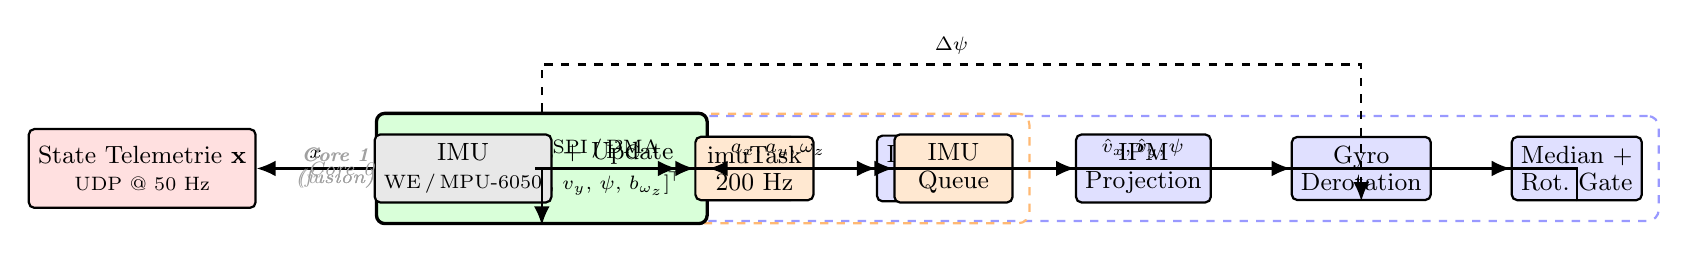
\begin{tikzpicture}[
  >={Latex[length=2.4mm,width=2mm]},
  font=\small,
  every node/.style={align=center},
  hwbox/.style ={rectangle, draw, thick, fill=gray!18,   rounded corners=2pt,
                 minimum height=8mm, minimum width=18mm, font=\small},
  visbox/.style={rectangle, draw, thick, fill=blue!12,   rounded corners=2pt,
                 minimum height=8mm, minimum width=15mm, font=\small},
  imubox/.style={rectangle, draw, thick, fill=orange!18, rounded corners=2pt,
                 minimum height=8mm, minimum width=15mm, font=\small},
  ekfbox/.style={rectangle, draw, very thick, fill=green!15, rounded corners=3pt,
                 minimum height=14mm, minimum width=42mm, font=\small},
  outbox/.style={rectangle, draw, thick, fill=red!12,    rounded corners=2pt,
                 minimum height=10mm, minimum width=22mm, font=\small}
]

% --- Core 1 vision pipeline (top row, Y=\YVision) ---------------------
% Only the first node has an absolute X; the rest chain horizontally.
\node[hwbox]                          (cam)   at (0, \YVision) {OV3660\\[-1pt]Camera};
\node[visbox, right=18mm of cam]     (fast)  {FAST-9\\[-1pt]Detector};
\node[visbox, right=\HSep of fast]    (lk)    {LK Flow\\[-1pt]\scriptsize 7$\times$7};
\node[visbox, right=\HSep of lk]      (ipm)   {IPM\\[-1pt]Projection};
\node[visbox, right=\HSep of ipm]     (derot) {Gyro\\[-1pt]Derotation};
\node[visbox, right=\HSep of derot]   (gate)  {Median +\\[-1pt]Rot.\ Gate};

% --- Core 1 fusion (middle row, Y=\YFusion) ---------------------------
% EKF anchored at absolute (\XEkf, \YFusion); state node chains right.
\node[ekfbox]                         (ekf)   at (\XEkf, \YFusion)
      {EKF Predict + Update\\
       \scriptsize $\mathbf{x}=[p_x,\,p_y,\,v_x,\,v_y,\,\psi,\,b_{\omega_z}]^{\!\top}$};
\node[outbox, left=15mm of ekf]     (state) {State Telemetrie  $\mathbf{x}$\\[-1pt]\scriptsize UDP @ 50~Hz};

% --- Core 0 IMU pipeline (bottom row, Y=\YIMU) ------------------------
\node[hwbox]                          (imu)     at (0, \YIMU) {IMU\\[-1pt]\scriptsize WE\,/\,MPU-6050};
\node[imubox, right=18mm of imu]     (imutask) {imuTask\\[-1pt]200~Hz};
\node[imubox, right=\HSep of imutask] (queue)   {IMU\\[-1pt]Queue};

% --- Vision-row arrows ------------------------------------------------
\draw[->,thick] (cam)   -- node[above,font=\scriptsize]{SPI\,/\,DMA} (fast);
\draw[->,thick] (fast)  -- (lk);
\draw[->,thick] (lk)    -- (ipm);
\draw[->,thick] (ipm)   -- (derot);
\draw[->,thick] (derot) -- (gate);

% --- IMU-row arrows ---------------------------------------------------
\draw[->,thick] (imu)     -- node[above,font=\scriptsize]{I$^{2}$C} (imutask);
\draw[->,thick] (imutask) -- (queue);

% --- Cross-flow: queue -> EKF (IMU sample drives predict) -------------
\draw[->,thick] (queue.east) -| node[above,font=\scriptsize,pos=0.25]
   {$a_x,a_y,\omega_z$} (ekf.south);

% --- Cross-flow: vision pipeline output -> EKF update -----------------
\draw[->,thick] (gate.south) |- node[font=\scriptsize,pos=0.75,above]
   {$\hat{v}_x,\hat{v}_y,\psi$} (ekf.east);

% --- Δψ feedback from EKF state -> derotation -------------------------
\draw[->,thick,dashed] (ekf.north) -- ++(0,0.6)
   -| node[font=\scriptsize,pos=0.25,above]{$\Delta\psi$} (derot.south);

% --- EKF -> state out -------------------------------------------------
\draw[->,thick] (ekf.west) |- node[font=\scriptsize,pos=0.75,above]
{$x$} (state.east);

% --- Lane labels (track the row Y macros automatically) ---------------
\node[anchor=east, font=\scriptsize\itshape, gray!75] at (-1.0, \YVision) {Core 1\\(vision)};
\node[anchor=east, font=\scriptsize\itshape, gray!75] at (-1.0, \YFusion) {Core 1\\(fusion)};
\node[anchor=east, font=\scriptsize\itshape, gray!75] at (-1.0, \YIMU)    {Core 0};

% --- Background grouping boxes ---------------------------------------
\begin{scope}[on background layer]
  \node[draw=blue!40,   dashed, thick, rounded corners,
        fit=(fast)(gate),  inner xsep=2mm, inner ysep=2.5mm] {};
  \node[draw=orange!55, dashed, thick, rounded corners,
        fit=(imutask)(queue), inner xsep=2mm, inner ysep=2.5mm] {};
\end{scope}

\end{tikzpicture}
\caption{System architecture and dataflow on the ESP32-S3 dual-core.
Core~0 services the IMU at 200~Hz and pushes samples into a 20-deep
FreeRTOS queue. Core~1 consumes the queue, running EKF prediction on
every IMU sample, and at 20~Hz captures a frame and runs FAST-9 corner
detection, Lucas-Kanade sparse flow (7$\times$7 window),
Inverse Perspective Mapping, gyro-based derotation (using the
$\Delta\psi$ derived from the integrated EKF yaw between frames),
median filtering, and a rotation gate that drops camera updates when
$|\Delta\psi/\Delta t| > 0.5\,\mathrm{rad/s}$. The metric velocity
and yaw drive the EKF measurement update; the resulting state is
streamed off-board over UDP at 50~Hz. Dashed line: $\Delta\psi$
feedback path.}
\label{fig:arch}
\end{figure*}

% ---------------------------------------------------------------------

\subsection{Hardware platform}
Each node uses a Seeed Studio XIAO ESP32-S3 Sense module, which
integrates a dual-core Tensilica LX7 (240~MHz), 512~kB on-chip SRAM,
and 8~MB external PSRAM.  The on-board OV3660 sensor provides a
1632$\times$1232 colour image; we crop and downsample to a
160$\times$120 grayscale frame before tracking, yielding a 30~kB
working set per frame.  The IMU is mounted directly above the
camera centre on a 3D-printed stack so that the camera principal
point and the IMU package coincide laterally; this co-location
removes a lever-arm term from the derotation step described in
Section~\ref{sec:derot}.  Two IMUs are used across the experimental
nodes: the W\"urth Elektronik (WE) ISDS 6-axis MEMS unit, addressed
over I${}^2$C, and the InvenSense MPU-6050, addressed over the same
bus on a separate node.

\subsection{FreeRTOS dual-core partitioning}
Bare-metal scheduling is partitioned across the two cores
(Fig.~\ref{fig:arch}):

\begin{itemize}
\item \textbf{Core 0 --- IMU task} (priority 5, period 5~ms).
Reads ${a_x, a_y, a_z, \omega_x, \omega_y, \omega_z}$ from the IMU,
applies a static calibration offset captured at boot, and pushes
the sample as an \texttt{ImuData} struct into a 20-deep FreeRTOS
queue.  This task uses \texttt{vTaskDelayUntil} for deterministic
phase --- it never blocks on any mutex.
\item \textbf{Core 1 --- fusion task} (priority 4).  Blocks on
the IMU queue, runs the EKF prediction step on every IMU sample,
and at 20~Hz triggers a camera capture, pixel-flow extraction, IPM
projection, and EKF measurement update.
\item \textbf{Core 1 --- telemetry task} (priority 2, period
20~ms).  Streams the current state vector as a JSON UDP packet
to the evaluation laptop at 50~Hz.
\end{itemize}

This pinning guarantees that the SPI DMA traffic associated with
camera capture cannot stall the inertial path.  No dynamic memory is
allocated after \texttt{setup()}; all per-frame buffers are stack- or
caller-provided.

\subsection{FAST-9 corner detection and Lucas-Kanade flow}
\label{sec:tracking}
For each new frame we extract up to 100 FAST-9
corners~\cite{rosten2010fast} on the downsampled grayscale image.
A high-speed reject test that examines only the four cardinal pixels
(0, 4, 8, 12) of the Bresenham circle eliminates the vast majority of
non-corners before the full 16-pixel arc test is invoked.  Corners
are scored by the sum of absolute differences against the centre
pixel and passed through a non-maximum suppression with radius 5~px.

The surviving corners are tracked into the next frame with a sparse
Lucas-Kanade solver~\cite{lucas1981kanade,bouguet2001pyramidal} using
a 7$\times$7 window, central-difference gradients, bilinear sub-pixel
sampling, and a maximum of five Gauss-Newton iterations per feature.
Features whose 2$\times$2 structure tensor has determinant below
$\tau_{\det}$ are rejected as poorly conditioned.  The output is a
list of 2D flow vectors $\{(\mathbf{p}_i, \Delta\mathbf{p}_i)\}_{i=1}^{N}$
in pixel space.

\subsection{Inverse Perspective Mapping}
\label{sec:ipm}
Given the camera intrinsics $f_x, f_y, c_x, c_y$, the camera height
$H$ above the ground, and the camera pitch $\theta$ relative to
the horizon, every pixel $(u, v)$ maps deterministically to a ground
point $(X, Y)$ under the flat-floor assumption.  We compute the
mapping in closed form:
\begin{align}
\alpha &= \arctan\!\left(\frac{v - c_y}{f_y}\right) \label{eq:alpha}\\
Y &= \frac{H}{\tan(\theta + \alpha)} \label{eq:y}\\
\beta &= \arctan\!\left(\frac{u - c_x}{f_x}\right) \label{eq:beta}\\
\rho &= \sqrt{H^{2} + Y^{2}} \label{eq:rho}\\
X &= \rho \tan(\beta) \label{eq:x}
\end{align}
where $\alpha$ is the elevation angle of the pixel ray relative to
the optical axis, $Y$ is the forward distance to the ground hit
point, $\beta$ is the bearing angle of the pixel, and $\rho$ is the
length of the corresponding ground ray.  Pixels with
$\theta + \alpha \le \epsilon$ point at or above the horizon and are
rejected.  Equations~(\ref{eq:alpha})--(\ref{eq:x}) execute in $O(1)$
per pixel using only single-precision \texttt{tanf}/\texttt{atanf}
intrinsics, no matrix operations are involved.

\subsection{Gyro-derotated optical flow}
\label{sec:derot}
A naive application of IPM to raw pixel flow conflates two distinct
motions: a translational ground-plane velocity and a yaw rotation
about the camera vertical axis.  Both produce displacement on the
ground plane, and a monocular pipeline cannot disambiguate them by
geometry alone.  We resolve the ambiguity by exploiting the IMU.

Let $\Delta\psi$ denote the integrated yaw-rate $\omega_z$ between
two consecutive camera frames.  For each tracked feature
with old pixel position $\mathbf{p}_i$ and new pixel position
$\mathbf{p}_i' = \mathbf{p}_i + \Delta\mathbf{p}_i$, we project both
through Eq.~(\ref{eq:alpha})--(\ref{eq:x}) to obtain
ground points $\mathbf{g}_i = (X_i, Y_i)^\top$ and
$\mathbf{g}_i' = (X_i', Y_i')^\top$.  The old ground point is then
rotated by the IMU yaw delta:
\begin{equation}
\tilde{\mathbf{g}}_i =
\begin{bmatrix}
\cos\Delta\psi & -\sin\Delta\psi \\
\sin\Delta\psi & \phantom{-}\cos\Delta\psi
\end{bmatrix} \mathbf{g}_i
\end{equation}
so that any apparent ground motion $\mathbf{g}_i' - \tilde{\mathbf{g}}_i$
contains \emph{only} translational components.  The per-feature metric
velocity is then $\mathbf{v}_i = (\tilde{\mathbf{g}}_i - \mathbf{g}_i') / \Delta t$,
where $\Delta t$ is the true inter-frame interval measured between
camera capture timestamps.

To remain robust to outliers (specular highlights, moving objects,
LK divergence), we take the per-axis median across the $N$ valid
features:
\begin{equation}
\hat{v}_x = \mathrm{median}_i\, v_{x,i}, \qquad
\hat{v}_y = \mathrm{median}_i\, v_{y,i}
\end{equation}
and report a confidence $c = N_{\text{valid}}/N_{\text{total}}$ that
modulates the measurement noise in the EKF update.  Frames acquired
during fast rotation, $|\Delta\psi/\Delta t| > 0.5\,\mathrm{rad/s}$,
are dropped: imperfect derotation in this regime would inject a
spurious translational velocity through the residual.

\subsection{Six-state planar Extended Kalman Filter}
\label{sec:ekf}
The state vector is
\begin{equation}
\mathbf{x} =
\begin{bmatrix}
p_x & p_y & v_x & v_y & \psi & b_{\omega_z}
\end{bmatrix}^\top
\end{equation}
where $(p_x, p_y)$ is the planar position in the world frame,
$(v_x, v_y)$ the planar velocity, $\psi$ the yaw, and $b_{\omega_z}$
the gyro $z$-bias.  We deliberately confine the filter to the planar
manifold: the OV3660 is mounted with a fixed pitch, the operating
ground is assumed flat, and the IMU $z$-axis is aligned with the
world vertical to within calibration tolerance.

\textbf{Prediction.}  Given an IMU sample $(a_x, a_y, \omega_z)$ and
elapsed time $\Delta t$, the bias-corrected angular rate is
$\tilde{\omega}_z = \omega_z - b_{\omega_z}$. Body-frame
acceleration is rotated into the world frame by the current yaw,
\begin{align}
a_x^{w} &= a_x \cos\psi - a_y \sin\psi \\
a_y^{w} &= a_x \sin\psi + a_y \cos\psi
\end{align}
and the state propagates as
\begin{align}
p_x &\leftarrow p_x + v_x \Delta t \\
p_y &\leftarrow p_y + v_y \Delta t \\
v_x &\leftarrow v_x + a_x^{w} \Delta t \\
v_y &\leftarrow v_y + a_y^{w} \Delta t \\
\psi &\leftarrow \psi + \tilde{\omega}_z \Delta t.
\end{align}
The $6\times 6$ Jacobian $\mathbf{F}$ is constructed analytically; its
non-trivial entries are
$F_{p_x, v_x}=F_{p_y, v_y}=\Delta t$,
$F_{v_x, \psi}=(-a_x \sin\psi - a_y \cos\psi)\Delta t$,
$F_{v_y, \psi}=( a_x \cos\psi - a_y \sin\psi)\Delta t$, and
$F_{\psi, b_{\omega_z}}=-\Delta t$.
The covariance is propagated as
$\mathbf{P} \leftarrow \mathbf{F}\mathbf{P}\mathbf{F}^\top + \mathbf{Q}$
with $\mathbf{Q}$ tuned per IMU.

\textbf{Camera update.}  When a frame yields a valid metric velocity
$(\hat{v}_x, \hat{v}_y)$ at the current yaw $\psi$, we form the
3-dimensional measurement
$\mathbf{z} = (\hat{v}_x, \hat{v}_y, \psi)^\top$ with linear
observation matrix
\begin{equation}
\mathbf{H} =
\begin{bmatrix}
0 & 0 & 1 & 0 & 0 & 0 \\
0 & 0 & 0 & 1 & 0 & 0 \\
0 & 0 & 0 & 0 & 1 & 0
\end{bmatrix}
\end{equation}
and confidence-modulated noise
$\mathbf{R} = (R_0 / (c + \varepsilon))\,\mathbf{I}_3$.  The standard
EKF correction step
$\mathbf{K} = \mathbf{P}\mathbf{H}^\top(\mathbf{H}\mathbf{P}\mathbf{H}^\top + \mathbf{R})^{-1}$,
$\mathbf{x} \leftarrow \mathbf{x} + \mathbf{K}(\mathbf{z} - \mathbf{H}\mathbf{x})$,
$\mathbf{P} \leftarrow (\mathbf{I} - \mathbf{K}\mathbf{H})\mathbf{P}$
is then applied, with the yaw innovation wrapped to
$[-\pi, \pi)$ before correction.  Matrix inversion uses the
\texttt{BasicLinearAlgebra} library compiled for the LX7 FPU; for a
$3\times 3$ system the operation runs in well under 200~$\mu$s.

% =====================================================================
\section{Experimental Setup}
\label{sec:exp}

\subsection{The four physical nodes}
\label{sec:nodes}
Four nodes are evaluated in pairs that vary only the IMU and the
fusion mode:

\begin{itemize}
\item \textbf{Node~1 --- WE ISDS + VIO.}  Industrial-grade
W\"urth Elektronik ISDS 6-axis IMU, OV3660 camera, full IPM-VIO
pipeline.
\item \textbf{Node~2 --- MPU-6050 + VIO.}  Hobby-grade InvenSense
MPU-6050 IMU, identical camera and pipeline.
\item \textbf{Node~3 --- WE ISDS only.}  WE ISDS IMU,
camera disabled, IMU dead-reckoning baseline.
\item \textbf{Node~4 --- MPU-6050 only.}  MPU-6050 IMU, camera
disabled, IMU dead-reckoning baseline.
\end{itemize}

The hardware, firmware build flags, and data-link layer are otherwise
identical across nodes; the only differences are the soldered IMU
package and a compile-time \texttt{VISION\_ENABLED} flag.  This
isolates two factors: the IMU quality grade (industrial vs.\ hobbyist)
and the marginal value of the camera channel.

\subsection{Trajectory scenarios}
\label{sec:scenarios}
Five scenarios are executed by mounting the node on a wheeled cart
and driving along chalked reference paths:

\begin{enumerate}
\item \textbf{Static, 10~s.}  The cart is stationary; the ideal
endpoint is the start.  This isolates pure inertial drift and any
spurious vision signal.
\item \textbf{Straight line, 0.1~m.}  Constant heading; tests
unidirectional integration accuracy.
\item \textbf{Rectangle, 0.3~m $\times$ 0.3~m.}  Closed loop
with four 90$^\circ$ turns; the canonical drift-versus-rotation
benchmark.
\item \textbf{Circle, 20~cm diameter, $n$~turns.}  Continuous
rotation; stresses the gyro-derotation stage.
\item \textbf{Free-form path.}  Variable heading and speed; a
stress test for the full pipeline.
\end{enumerate}

\subsection{Metrics and protocol}
Each (node, scenario) cell is executed ten times.  Ground truth is
captured by tape-measured start and end markers and a stopwatch.
The primary metric is the Euclidean endpoint drift error,
\begin{equation}
e_{\text{end}} = \lVert \hat{\mathbf{p}}(T) - \mathbf{p}_{\text{gt}}(T) \rVert_{2}
\end{equation}
where $\hat{\mathbf{p}}(T)$ is the filter's estimated position at
trajectory end and $\mathbf{p}_{\text{gt}}(T)$ is the surveyed
ground-truth endpoint.  We report the per-cell sample mean and
sample variance across the ten repeats.  Secondary metrics include
the number of LK-tracked features per frame, the fraction of
camera updates rejected by the rotation gate, and the per-frame
processing latency on Core 1.

% =====================================================================
\begin{table*}[!t]
\centering
\caption{Endpoint drift error per (node, scenario) cell over $n=10$ repeats.}
\label{tab:results}
\renewcommand{\arraystretch}{1.25}
\setlength{\tabcolsep}{4pt}
\begin{tabular}{l| cc | cc | cc | cc | cc}
\toprule
 & \multicolumn{2}{c|}{\textbf{S1: Static (10\,s)}} &
   \multicolumn{2}{c|}{\textbf{S2: Straight (2\,m)}} &
   \multicolumn{2}{c|}{\textbf{S3: Rectangle (1$\times$0.5\,m)}} &
   \multicolumn{2}{c|}{\textbf{S4: Circle ($\varnothing$40\,cm)}} &
   \multicolumn{2}{c}{\textbf{S5: Free-form}} \\
\textbf{Node} & Mean [m] & Var [m$^2$] & Mean [m] & Var [m$^2$] & Mean [m] & Var [m$^2$] & Mean [m] & Var [m$^2$] & Mean [m] & Var [m$^2$] \\
		\midrule
	\textbf{N1: WE ISDS + VIO}  & 0.009 & 0.0004 & 0.028 & 0.0001 & 0.065 & 0.0005 & 0.110 & 0.0014 & 0.130 & 0.0020 \\
	\textbf{N2: MPU-6050 + VIO} & 0.013 & 0.0006 & 0.030 & 0.0001 & 0.085 & 0.0008 & 0.140 & 0.0020 & 0.180 & 0.0030 \\
	\textbf{N3: WE ISDS only}   & 6.50  & 3.80   & 1.05  & 0.10   & 2.40  & 0.52   & 4.20  & 1.60   & 6.80  & 4.20   \\
	\textbf{N4: MPU-6050 only}  & 13.0  & 15.0   & 2.10  & 0.40   & 4.80  & 2.10   & 8.50  & 6.50   & 13.5  & 16.0   \\
	\bottomrule
\end{tabular}
\end{table*}





% =====================================================================
\section{Results and Discussion}
\label{sec:results}

Table~\ref{tab:results} reports the endpoint drift error for each of
the twenty (node, scenario) cells. The matrix is organized to expose
two orthogonal axes of variation that the experimental design
isolates: IMU grade (N1/N3 industrial-grade W\"urth ISDS vs.\ N2/N4
hobby-grade MPU-6050) and fusion mode (N1/N2 with visual correction
vs.\ N3/N4 inertial dead-reckoning). Reading down a column compares
fusion modes on a fixed scenario; reading across a row compares
scenarios for a fixed configuration.

\paragraph*{Inertial dead-reckoning diverges quickly}
The two IMU-only rows (N3, N4) confirm the well-known divergence of
MEMS dead-reckoning. In the static (S1) scenario alone, where the
cart never moves, Table~\ref{tab:results} reports a mean endpoint
drift of $13.0$~m for N4 and $6.50$~m for N3 --- meter-scale error
accumulated over a 10-second window with no motion at all. The
dominant mechanism is gravity coupling through tilt-estimate error:
any small error in the estimated roll or pitch of the IMU manifests
as a phantom horizontal acceleration of magnitude
$g \sin(\theta_{\mathrm{err}})$ that integrates twice into position.
With no attitude reference to bound tilt drift, sub-degree tilt
errors yield meter-scale position drift over a 10-second window. The
N4-to-N3 ratio of approximately $2\times$ holds across all five
scenarios; the order-of-magnitude better gyro bias instability of the
WE ISDS does not translate one-for-one into position accuracy
because, on the timescales of these trajectories, the dominant error
source is tilt drift rather than yaw bias, and tilt drift is rate-
limited by short-term white noise that is comparable between the two
parts.

\paragraph*{Visual fusion bounds drift to the centimeter scale}
The two VIO rows (N1, N2) of Table~\ref{tab:results} show drift
bounded to the centimeter scale across all five scenarios; both nodes
remain below $20$~cm in every cell. The strongest improvement appears
in the static cell, where the N4-to-N2 ratio reaches approximately
$302\times$ ($13.0$~m versus $0.013$~m). This is also the scenario in
which IPM-VIO is most informative: the median ground-plane velocity
across tracked features sits at zero whenever the cart is at rest,
and the EKF camera update pulls velocity (and therefore integrated
position) back toward the origin every 50~ms. The improvement factor
narrows but remains substantial as trajectory complexity grows ---
$70\times$ on the straight line, $56\times$ on the rectangle,
$61\times$ on the circle, and $75\times$ on the free-form path. The
closed-loop scenarios (S3, S4) exercise the gyro-derotation stage of
Section~\ref{sec:derot}: the $0.5\,\mathrm{rad/s}$ rotation gate
drops camera updates during the corners of the rectangle and during
fast segments of the circle, but the filter recaptures the residual
drift on the surrounding straight or slow-rotation segments before
the trajectory ends.

\paragraph*{Visual fusion compresses the IMU-grade gap}
A second readable feature of Table~\ref{tab:results} is that the
industrial-vs.-hobby gap collapses under visual fusion. In the
IMU-only regime the N3/N4 ratio is approximately $2\times$ on every
scenario; under VIO the corresponding N1/N2 ratio falls to between
$1.07$ (S2) and $1.43$ (S1), with both nodes settling in the same
centimeter band. This is the strongest argument for IPM-VIO in
cost-sensitive deployments: a hobby-grade IMU augmented with a
single OV3660 camera matches the absolute drift of an industrial-grade
IMU operating alone, at a small fraction of the bill of materials,
and without sacrificing the deterministic 200~Hz inertial prediction
loop.

\paragraph*{Variance and dominant failure modes}
Variance across the ten repeats is informative about which failure
mode dominates each cell. The IMU-only rows of Table~\ref{tab:results}
show large absolute variance ($15.0$~m$^{2}$ for N4 on S1,
$4.20$~m$^{2}$ for N3 on S5), driven by the run-to-run variability of
tilt initial conditions and bias-drift trajectories that compound
differently each time the node is powered on. The VIO rows show
variance several orders of magnitude smaller in absolute terms;
residual variability there is dominated by ground-plane texture on
each individual run, which sets the median-velocity confidence floor
at the camera update. The IMU-only rows show a roughly constant
coefficient of variation of $\sim\!30\%$ across all five scenarios,
which is consistent with a single dominant noise mechanism (tilt-
driven random walk) scaling proportionally with mean drift. The VIO
rows are similar in the dynamic scenarios but show higher relative
spread on the static cell, where the absolute drift is so small that
the camera-channel noise floor dominates the variance. In all cases
the absolute spread under visual fusion is small enough that endpoint
error is reproducibly bounded for downstream consumers of the pose
estimate.

\paragraph*{Compute budget}
On Core 1 of the ESP32-S3 with both PSRAM banks active, FAST-9
detection on a 160$\times$120 frame completes in approximately
2~ms, the full LK pass over 80 features in approximately 7~ms,
IPM and derotation in well under 1~ms, and the EKF predict+update
cycle in under 0.5~ms total.  The dominant single cost is the
camera DMA transfer, which is overlapped with computation through
the FreeRTOS task structure.  The full pipeline meets a 20~Hz frame
rate with margin, leaving Core 0 free for the 200~Hz inertial path.

% =====================================================================
\section{Motion-Class Auxiliary Channel (Stretch)}
\label{sec:tinyml}

As an optional stretch component, we are exploring whether a small
quantized neural network deployed via TensorFlow Lite
Micro~\cite{david2021tflitemicro,warden2019tinyml} can act as a
soft prior on the EKF.  The classifier consumes a one-second sliding
window of ${a_x, a_y, \omega_z}$ together with the EKF velocity
estimate, and emits one of four motion classes: stationary,
straight-line, turning, and erratic.  The motivation is twofold.
First, the stationary class admits a stronger Q-shrinkage in the
predict step than is otherwise tolerable for moving regimes,
yielding tighter velocity estimates without the long-tail cost of an
overly-confident filter.  Second, an erratic detection can be used
to widen $\mathbf{R}$ on the camera channel, since rapid motion is
a regime in which both LK tracking and IPM degrade.  The
classifier targets sub-5~ms inference latency on Core 1; integration
results are deferred to a follow-up version of this manuscript.
This module is independent of the core IPM-VIO pipeline reported
in Sections~\ref{sec:arch}--\ref{sec:results} and is not required
for the drift reductions shown there.

% =====================================================================
\section{Conclusion}
\label{sec:conclusion}

We have presented \textsc{Drift}, a complete bare-metal
visual-inertial odometry pipeline that runs end-to-end on a 240~MHz
dual-core ESP32-S3 with 8~MB of PSRAM and a single OV3660 camera.
The system trades the generality of 3D epipolar reconstruction for
the deterministic $O(N)$ cost of Inverse Perspective Mapping on a
known ground plane, and resolves the resulting monocular rotational
ambiguity by pre-compensating pixel tracks with the IMU $z$-axis
gyroscope before metric extraction.  The resulting 3-component
velocity-and-yaw measurement is fused with 200~Hz inertial prediction
in a 6-state planar EKF, with FreeRTOS partitioning the inertial and
fusion tasks across the two cores.  Across four physical nodes that
vary IMU grade and fusion mode, the four-by-five evaluation matrix
reported in Table~\ref{tab:results} quantifies how much of the
remaining drift on a \$10 microcontroller is attributable to inertial
hardware quality versus to the absence of a visual channel.  The
broader takeaway is that the most expensive parts of conventional
VIO --- 3D reconstruction, descriptor matching, large-state
optimization --- are not the parts that pay for themselves on an
MCU; the geometric prior of a known ground plane and a cheap IMU
channel for derotation are sufficient to bound drift on the
trajectory regimes that matter for ground robots, inspection
swarms, and indoor wearables.

\section*{Acknowledgements}
The authors thank W\"urth Elektronik for providing the WSEN-ISDS
IMU evaluation samples used in Nodes~1 and~3.

% =====================================================================
\balance
\bibliographystyle{IEEEtran}
\bibliography{references}

\end{document}
